\documentclass{article}

\title{Informe de Laboratorio}

%%%%%%%%%%%%%%%%%%%%%%%%%%%%%%%%%%%%%%%%%%%%%%%%%%%%%%%%%%%%%%%%%%%%%%%%%%%%
%%%%%%%%%%%%%%%%%%%%%%%%%%%%%%%%%%%%%%%%%%%%%%%%%%%%%%%%%%%%%%%%%%%%%%%%%%%%
\newcommand{\itemEmail}{vsullaq@unsa.edu.pe}
\newcommand{\itemStudent}{VLADIMIR ARTURO SULLA QUISPE}
\newcommand{\itemTeacher}{CARLO JOSE LUIS CORRALES DELGADO}
\newcommand{\itemGitHubURL}{https://github.com/Vladimir2003-debug/PW2-LAB04.git}
\newcommand{\itemCourse}{PROGRAMACION WEB 2}
\newcommand{\itemCourseCode}{20231001}
\newcommand{\itemSemester}{III}
\newcommand{\itemUniversity}{Universidad Nacional de San Agustín de Arequipa}
\newcommand{\itemFaculty}{Facultad de Ingeniería de Producción y Servicios}
\newcommand{\itemDepartment}{Departamento Académico de Ingeniería de Sistemas e Informática}
\newcommand{\itemSchool}{Escuela Profesional de Ingeniería de Sistemas}
\newcommand{\itemAcademic}{2023 - A}
\newcommand{\itemInput}{}
\newcommand{\itemOutput}{}
\newcommand{\itemPracticeNumber}{04}
\newcommand{\itemTheme}{PYTHON}
%%%%%%%%%%%%%%%%%%%%%%%%%%%%%%%%%%%%%%%%%%%%%%%%%%%%%%%%%%%%%%%%%%%%%%%%%%%%
%%%%%%%%%%%%%%%%%%%%%%%%%%%%%%%%%%%%%%%%%%%%%%%%%%%%%%%%%%%%%%%%%%%%%%%%%%%%

% COLORS

%Paquetes 
\usepackage{graphicx} % Required for inserting images
\usepackage{array}
\usepackage{multirow}
\usepackage[top=3cm, bottom=3cm, outer=3cm, inner=3cm]{geometry}
\usepackage[document]{ragged2e}
\setlength{\headheight}{30pt}
\usepackage{colortbl}
\graphicspath{ {images/} }
\usepackage{listings}
\lstdefinestyle{ascii-tree}{
    literate={├}{|}1 {─}{--}1 {└}{+}1 
  }
\lstset{basicstyle=\ttfamily,
  showstringspaces=false,
  commentstyle=\color{red},
  keywordstyle=\color{blue}
}
\usepackage[utf8]{inputenc}

\usepackage{fancyhdr}
\pagestyle{fancy}
\fancyhf{}
\setlength{\headheight}{30pt}
\renewcommand{\headrulewidth}{1pt}
\renewcommand{\footrulewidth}{1pt}
\fancyhead[L]{\raisebox{-0.2\height}{\includegraphics[width=3cm]{img/logo_episunsa.png}}}
\fancyhead[C]{\fontsize{7}{7}\selectfont	\itemUniversity \\ \itemFaculty \\ \itemDepartment \\ \itemSchool \\ \textbf{\itemCourse}}
\fancyhead[R]{\raisebox{-0.2\height}{\includegraphics[width=1.2cm]{img/logo_abet}}}
\fancyfoot[L]{\itemEmail }
\fancyfoot[C]{\itemCourse}
\fancyfoot[R]{Página \thepage}


\begin{document}

\vspace*{30px}

\begin{center}	
		\fontsize{17}{17} \textbf{ Informe de Laboratorio \itemPracticeNumber}
\end{center}
 
\renewcommand{\arraystretch}{1.5}
\begin{tabular}{ |l|l|l|l|l|l| }
    \hline
    
    \multicolumn{6}{|c|}{\cellcolor{red}INFORMACIÓN BÁSICA} \\
    \hline
    ASIGNATURA: & \multicolumn{5}{|l|}{ \itemCourse} \\
    \hline
    TITULO DE LA PRÁCTICA: & \multicolumn{5}{|l|}{\itemTheme} \\
    \hline     
    NÚMERO DE PRÁCTICA: & 04 & AÑO LECTIVO: & 2023-A & NRO. SEMESTRE: & \itemSemester\\
    \hline     
    FECHA DE PRESENTACIÓN & 08/06/23 & HORA DE PRESENTACIÓN: & \multicolumn{3}{|l|}{ 00:00 } \\
    \hline     
    \multicolumn{4}{|l|}{INTEGRANTE (s): 
    - \itemStudent 
    } &  NOTA (0-20) & \\
    \hline
    \multicolumn{6}{|l|}{GITHUB :\itemGitHubURL} \\
    \hline
    \multicolumn{6}{|l|}{DOCENTE(s): 
    - \itemTeacher 
    } \\
    \hline     
\end{tabular}

\section{TAREA}
Implemente los métodos de la clase Picture. Se recomienda que implemente la clase picture por etapas, probando realizar los dibujos que se muestran en la siguiente preguntas.

Usando únicamente los métodos de los objetos de la clase Picture dibuje las siguientes figuras (invoque a draw):

\begin{itemize}
    \item a.\\ 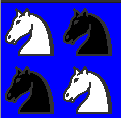
\includegraphics{img/ejercicio_02_a.png} 
    \item b.\\ 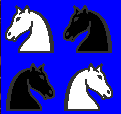
\includegraphics{img/ejercicio_02_b.png} 
    \item c.\\ 
\includegraphics{img/ejercicio_02_c.png}   \item d.\\ 
\includegraphics{img/ejercicio_02_d.png} 
    \item e.\\ 
\includegraphics{img/ejercicio_02_e.png} 
    \item f.\\ 
\includegraphics{img/ejercicio_02_f.png} 
    \item g.\\ 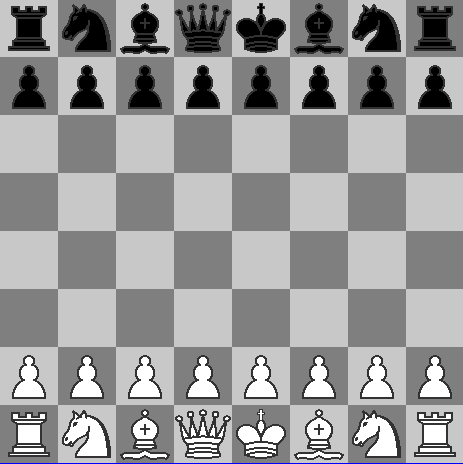
\includegraphics{img/ejercicio_02_g.png} 
\end{itemize}

\section{MATERIALES USADOS}

\begin{itemize}
    \item Sistema Operativo Windows 10 Home Single Language
    \item Python 3.10.4
    \item virtualenv 20.14.1
    \item pygame 2.4.0
    \item Cuenta de GitHub
\end{itemize}

\section{ORGANIZACION Y ESTRUCTURA DEL LABORATORIO}
\begin{itemize}	
		\item El contenido que se entrega en este laboratorio es el siguiente:
\end{itemize}
 
\begin{lstlisting}[style=ascii-tree]
PW2 LAB04/
    |--- __pycache__
    |--- env/
    |--- img
        |--- logo_abet.png
        |--- logo_episunsa.png
        |--- logo_unsa.jpg
    |--- .gitignore
    |--- chessPictures.py    
    |--- colors.py    
    |--- Ejercicio2a.py
    |--- Ejercicio2b.py
    |--- Ejercicio2c.py
    |--- Ejercicio2d.py
    |--- Ejercicio2e.py
    |--- Ejercicio2f.py
    |--- Ejercicio2g.py
    |--- picture.py
    |--- pieces.py
    |--- README.md
    |--- requirements.py
    |--- Test.py

\end{lstlisting}    

\section{SOLUCION}
\begin{itemize}
    \item Primero Solucionamos los metodos de la clase picture. Usamos la figura knight para evaluar si se mueve a la izquierda o la derecha \\

    \lstinputlisting[language=Python, caption={picture.py},numbers=left,]{picture.py}

    \item Luego solo es cuestion de resolver los ejercicios jugando con los metodos picture \\

    \item Ejercicio2a.py \\
    \lstinputlisting[language=Python, caption={Ejercicio2a.py},numbers=left,]{Ejercicio2a.py}

        \item Ejercicio2b.py \\
    \lstinputlisting[language=Python, caption={Ejercicio2b.py},numbers=left,]{Ejercicio2b.py}

        \item Ejercicio2c.py \\
    \lstinputlisting[language=Python, caption={Ejercicio2c.py},numbers=left,]{Ejercicio2c.py}

        \item Ejercicio2d.py \\
    \lstinputlisting[language=Python, caption={Ejercicio2d.py},numbers=left,]{Ejercicio2d.py}

        \item Ejercicio2e.py \\
    \lstinputlisting[language=Python, caption={Ejercicio2e.py},numbers=left,]{Ejercicio2e.py}

        \item Ejercicio2f.py \\
    \lstinputlisting[language=Python, caption={Ejercicio2f.py},numbers=left,]{Ejercicio2f.py}

        \item Ejercicio2g.py \\
    \lstinputlisting[language=Python, caption={Ejercicio2g.py},numbers=left,]{Ejercicio2g.py}
    
    
\end{itemize}


\section{CUESTIONARIO}

\begin{itemize}
    \item ¿Qué son los archivos *.pyc?  \\
    Los archivos PYC son utilizados por el lenguaje de programación Python. PYC es un archivo ejecutable que contiene el código de bytes compilado para un programa escrito en Python. Bytecode es un conjunto de instrucciones para que el intérprete ejecute el programa. Basicamente son el archivo .py pero en version de codigos de bytes
    
    \item ¿Para qué sirve el directorio pycache? \\
    Cuando el interprete de python ejecuta archivos .py lo compila en codigo de bytes y lo almacena en el directorio pycache con extension .pyc para que a la siguiente que se ejecute el archivo no tenga que volver a hacer el mismo procedemiento. 
    
    \item ¿Cuáles son los usos y lo que representa el subguión en Python? \\
    El guion bajo se usa para evitar conflictos con palabras clave o elementos.
    
\end{itemize}

\section{REFERENCIAS}

\begin{itemize}
    \item \url {https://www.w3schools.com/python/python_reference.asp} \\ 
    \item \url{https://docs.python.org/3/tutorial/}\item \url{https://www.file-extension.info/es/format/pyc}
    \item \url{https://stackoverflow.com/questions/16869024/what-is-pycache}
    \item \url{https://frankgalandev.com/que-significa-el-guion-bajo-en-python/#:~:text=Se%20utiliza%20para%20evitar%20conflictos,con%20elementos%20integrados%20en%20Python.&text=En%20este%20caso%20indica%20que,este%20aspecto%20de%20su%20implementaci%C3%B3n.}
\end{itemize}


\end{document}
